\documentclass[12pt]{ctexart}
\usepackage{amsmath, CJKutf8, setspace, tabu, multirow, fancyhdr, indentfirst, geometry, graphicx, color, xcolor, ulem, hyperref}
\hypersetup{
    colorlinks=true,
    linkcolor=blue,
    filecolor=blue,      
    urlcolor=blue,
    citecolor=cyan,
}

\geometry{left=3cm,right=3cm,top=3.0cm,bottom=3.0cm}

\setCJKmainfont[BoldFont=STKaiti]{KaiTi}
\begin{document}

\pagestyle{fancy}
\lhead{2020年普通高等学校招生全国统一考试}
\rhead{Solution}
\renewcommand{\headrulewidth}{0.4pt}
\date{\today}
\author{huangkui}
\title{Solution}

\begin{spacing}{1.2}
    \maketitle

	\newpage

	\section{物理}
	
	\subsection{题意}
	给你一张$n$个点, $m$条边的无向图, 边权为$2^k$, 求$S$到$T$的最短路

	\subsection{题解}

	先考虑$k$互不相等的情况: 

	每经过一条边, dis只会增加$2^k$. 当$k$互不相等时, 不会发生进位, 于是可以在做最短路时, 用主席树来储存答案, 每次把一个$0$修改成$1$即可. 至于比较大小, 可以通过hash来找出第一个不相同的位置
	\\


	没有$k$互不相等的条件时, 就有可能发生进位. 当发生进位时, 暴力地找出连续的一段$1$变成$0$, 然后将一个$0$变成$1$即可
	\\

	复杂度证明:  

	设势能函数为当前状态下$1$的个数. 一次操作要么最多增加$1$个$1$, 要么消耗当前的若干个$1$, 所以总复杂度是关于操作次数线性的
	\\

	线段树模拟即可, 时间复杂度$O(n\log^2 n)$

	\newpage

	\section{化学}

	\subsection{题意}
	给一棵$n$个点的树, 有$m$次询问. 每次询问给出$x$, 求一个最小的$k$使得把树上$k$条边断掉然后重新连$k$条边形成一棵新的树之后, 树的重心为$x$

	\subsection{题解}

	重心的一个性质: 

	\begin{itemize}
	\item 以$x$为根时每棵子树的$size$都$\le \frac{n}{2}$, 是$x$为重心的充要条件
	\end{itemize}

	充分性: 走到$x$的某一个儿子节点, 那么$x$所在子树的$size$就$ > \frac{n}{2}$

	首先, 重心的答案为$0$, 然后考虑求出以重心为根时, 至少要删掉多少个儿子才能使得剩下的节点数$\le \frac{n}{2}$

	那么答案要么是这个值, 要么是它减一

	举个例子: 

	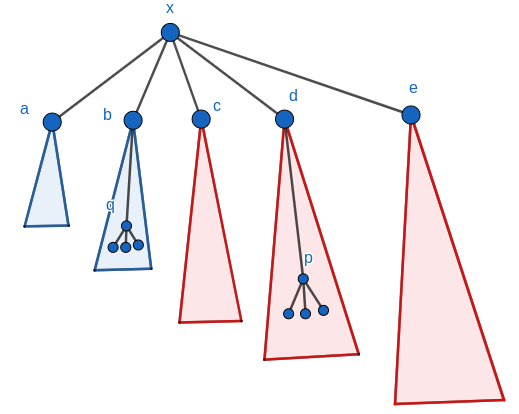
\includegraphics[width=0.6\linewidth]{image/1.png}

	假设至少需要删掉$c, d, e$三个儿子才能使得剩下节点数$\le \frac{n}{2}$

	\begin{itemize}

	\item 考虑一个在$d$子树中的点$p$的答案, 首先至少要删掉$c, e$两棵子树, 然后通过计算剩下部分(全集去掉$p、c、e$的子树)的大小是否$\le \frac{n}{2}$来判断是否需要+1

	\item 考虑一个在$b$子树中的点$q$的答案, 首先至少要删掉$d, e$两棵子树, 然后通过计算剩下部分(全集去掉$q、d、e$的子树)的大小是否$\le \frac{n}{2}$来判断是否需要+1

	模拟即可, 时间复杂度$O(n)$

	\end{itemize}

	\newpage

	\section{生物}

	\subsection{写在前面}
	\href{https://loj.ac/article/567}{https://loj.ac/article/567}

	官方认证,思维难度提高+, 实现难度提高

	\subsection{题意}
	你有一个长为$n$的序列, 每个位置是 $*$ 或者 $+$, $*$ 表示让变量加上自身, $+$ 表示让变量$+1$

	你要选出它的一个子序列, 使得一个初始为$0$的变量在对子序列中的字符依次执行对应操作后对$2^k$取模所得结果尽可能大. 求出最大可能的结果. 

	\subsection{题解}

	不难发现, 在最终的答案序列中, 每个$+$对答案的贡献为$2^d$ ($d$表示这个$+$后面的$*$数量). 贪心地考虑, 如果能想办法使得$+$后面的$*$更多, 那么答案会更优. 

	注意到$*+++$与$+*+$是等价的, 我们只需要不断进行这样的变换操作, 即能把原串变成一个新串, 满足相邻两个$*$之间没有两个以上的$+$

	记$a[i]$表示有多少个$+$号满足它后面有$i$个$*$, 从答案的高位往低位考虑, 找到第一个满足$a[i]=0$的位$p$(若找不到则答案为$2^k-1$), 那么高于$p$的位都能为$1$, 低于$p$的位剩下的$+$和$*$都能选(因为即使全选也不会在$p$这一位产生进位, 所以都能选)

	模拟即可, 时间复杂度$O(n)$

	\newpage

\end{spacing}

\end{document}
